\documentclass[a4paper]{book}
\usepackage[utf8]{inputenc}
\usepackage[margin=3cm]{geometry}
\usepackage{appendix, tikz, pgfplots, graphicx, pdfpages}

\pgfplotsset{width = \textwidth, compat = newest}


\begin{document}
\begin{titlepage}
    \begin{center}
        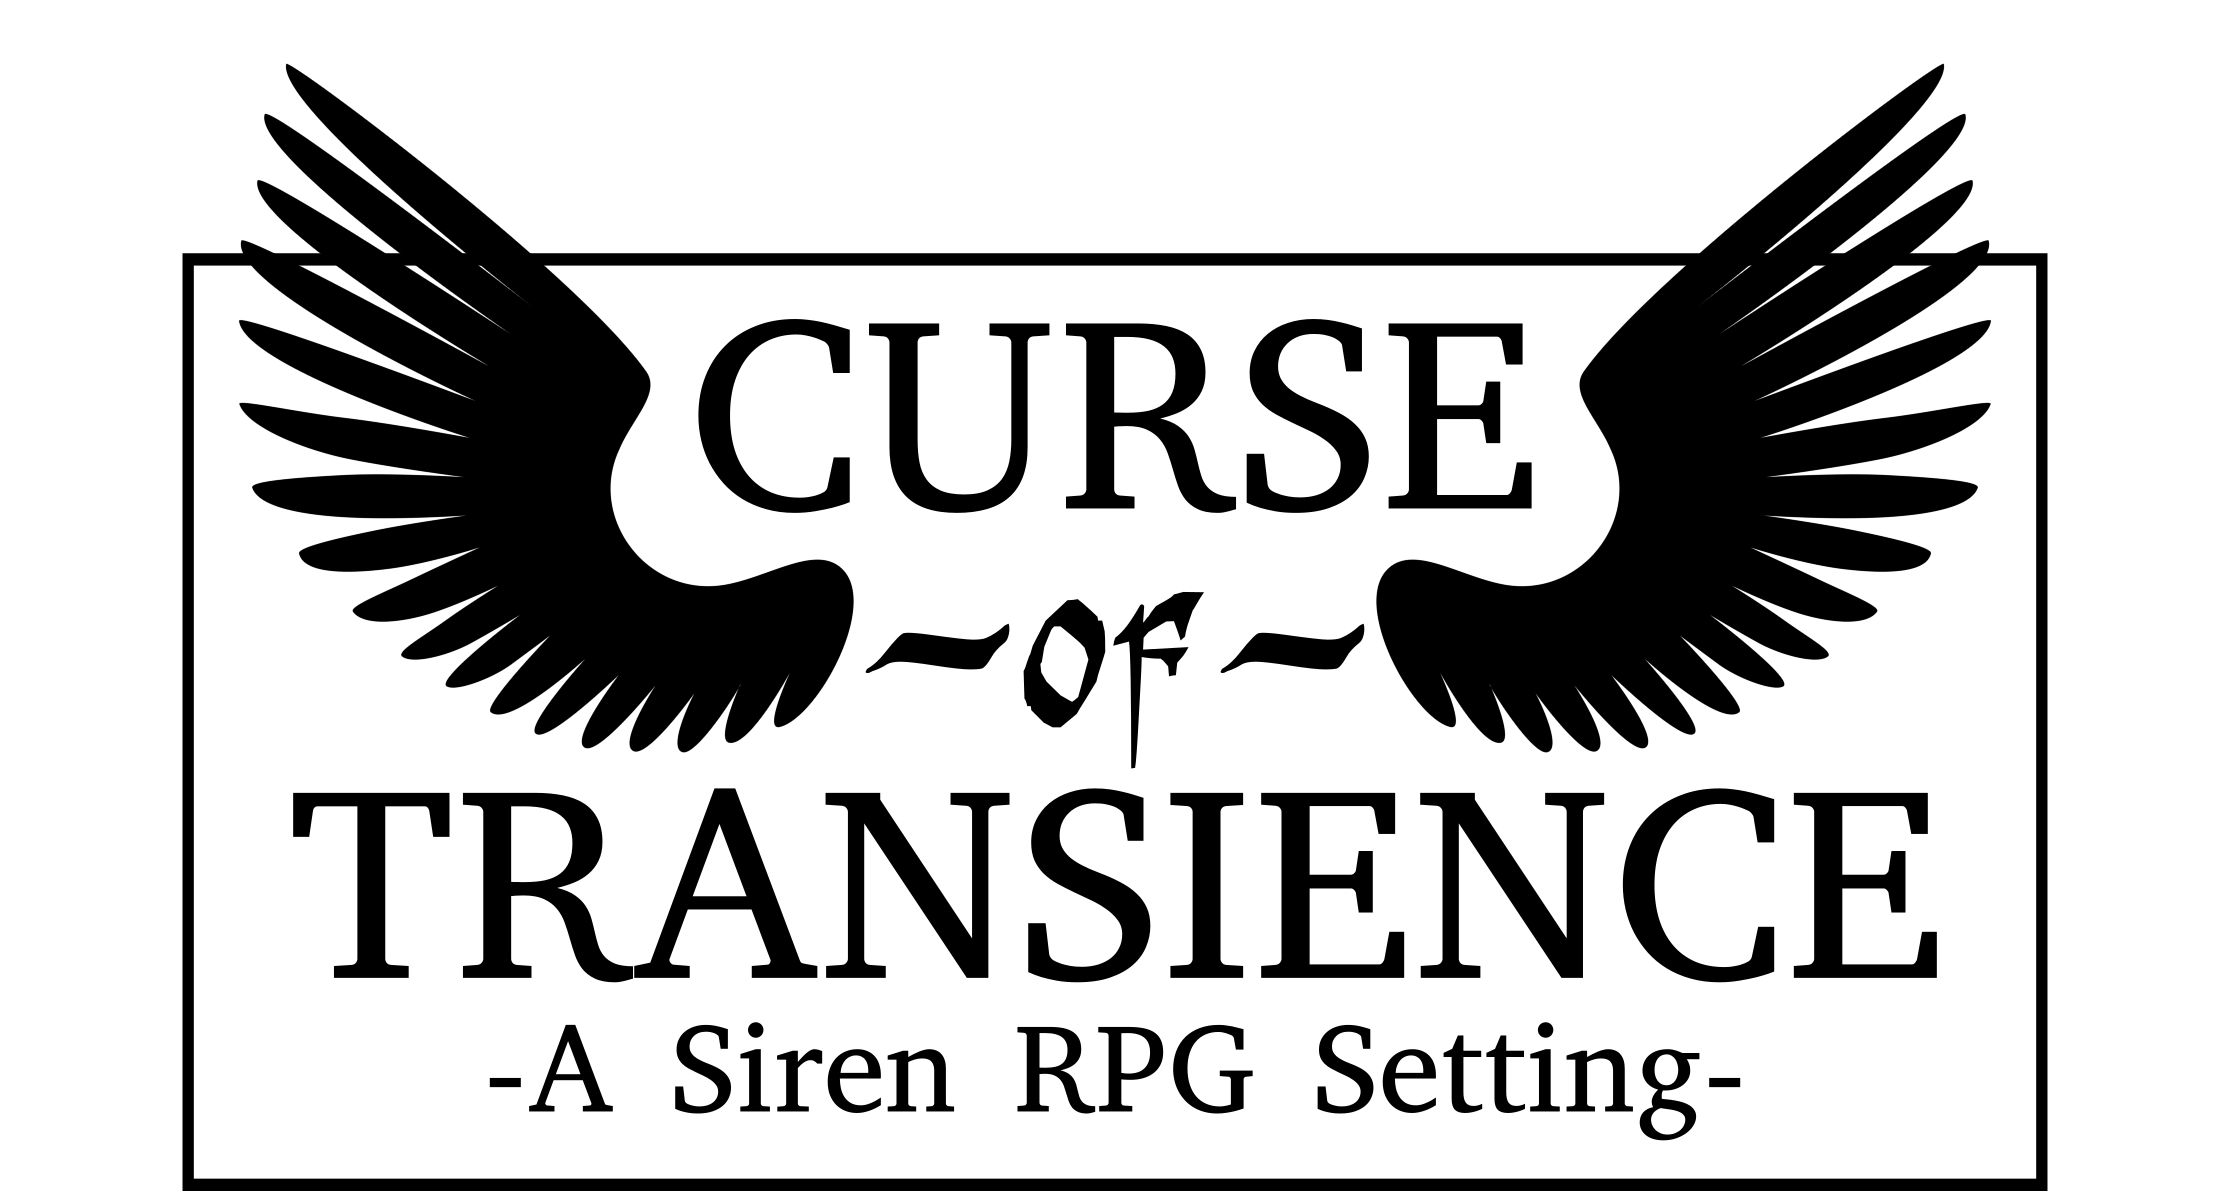
\includegraphics[width = \textwidth]{graphics/logo-winged.png}
    \end{center}
\end{titlepage}
\thispagestyle{empty}
\frontmatter
\begin{center}
    \Huge{Curse of Transience}\\
    \Large{By Alex Laterman \& Niko Lepka}\\
    \large{\today}
\end{center}

\chapter*{Preface}
\textit{The Curse of Transience} is a worldbook for the \textit{Siren} role-playing system\footnote{\texttt{https://github.com/ElectricCoffee/SirenRPG}}, and thus does not act as a self-contained document.
If you're going to use this setting in a campaign, we recommend you familiarise yourself with that first.

\chapter*{Introduction}

\tableofcontents
\mainmatter
\part{You, The Player}
% Character Creation
\chapter{Character Creation}

% Races
\chapter{Races}\label{chap:races}
\section{Humans}
Your standard garden variety person.
Comes in all sorts of shapes, sizes and colours.
Generally lazy, yet territorial.
\section{Trolds -- Woodland Trolls}
Woodland trolls---often simply called \textit{Trolds}---hail from the colder regions of the world and have lived peacefully in societies parallel to humans for centuries.
It is not uncommon for Woodland trolls to be found living and working in human cities, but tend to keep to burrow-communities in the various forests.

\paragraph{Physical Description}
Trolds are relatively short for trolls, adults typically ranging from around 1.3m to around 1.6m.
Trolds have tails, long enough to reach the floor from a standing position, ending in a tuft of hair.
Like humans, trolls have five fingers on each hand and five toes on each foot, though unlike humans they have long pointy ears and small horns purtruding through their hair.
Troll body hair is also thicker than that found on humans.

Trolds have fair skin and thus easily get sunburnt, though unlike their mountainous counterparts (see~Section~\ref{sec:trolls}), they do not turn to stone in direct sunlight.
And while not blinded by direct sunlight, they do possess quite good night-vision.

Life-expectancy for a trold is around 130--240 years.

\paragraph{Society}
Trold usually live in family burrows spread across the various forests across the world.
Burrows usually have a population of 15-30 individuals, typically lead by the oldest matriarch or matriarchs in the burrow. 
This matriarch is referred to as \textit{Mother}.
The largest burrow recorded in Saoghall history has had 97 trolls living within.
As such, trolds do not usually create \textit{troll countries}, but rather try to integrate---if possible---into the existing surrounding societies.

The vast majority of trolds commit to a ceremonial topside journey---called \textit{The Exodus}---from their burrow, usually as a coming-of-age period or as a means of bringing in new skills and trades into the burrow.
Most trolds return to their burrows after a few years, but some choose to stay topside for the remainder of their lives.
The purpose of this exodus is threefold; it can thin out the population of a burrow so it doesn't become overcrowded, it brings new blood into the burrow by having the trolds return with a mate, or it brings in new ways and means into the burrow by having trolds learn new trades topside.

Just about every burrow in the world has an exodus, but this is usually motivated differently for each.

\paragraph{Relations}
While most trold burrows are isolated by their nature, their relation to the outside world varies wildly from friendly, to cautious, to outright xenophobic.

The practice of The Exodus is known to have caused problems within certain human societies, as the the influx ``outsiders'' to human villages and cities sometimes causes them receive blame for preceived economic pressure.

\paragraph{View on the Undead}
Trolds are generally uncomfortable with undeath.
Those living topside typically have a begrudging tolerance towards undeath, and will deal with it if need be, but those living in burrows are typically less keen on it.
Most burrows are not happy about trolds returning from The Exodus in a state of visible undeath, and---if signs are clear enough---will outright refuse the trold to return.

\paragraph{Religion}
Most trolds will worship the spirits of their local forest, generally focusing on a guardian figure local to their climate, though trolds born and raised in cities will sometimes adopt the local religion.

\paragraph{Adventurers}
As a natural consequence of The Exodus, many trolds choose to become adventurers to broaden their world view and acquire new skills.

\paragraph{Names}
Trolls have a relatively strict and complex naming convention.

The general pattern is \textsc{[first-name]}, \textsc{[occupation]} of \textsc{[burrow-name]}. \\For example: \textit{Janice, Tailor of Wierwood Warren}.

However, if a Trold has not yet gone on their Exodus, they typically use their parent's occupation and their relation to them:\\
For example: \textit{Ghorm, Fletcherson of Smokey Woods Hollow}.

Note that being the elder of a burrow is considered an occupation, thus \textit{Mother}, \textit{Father}, or \textit{Elder} are used in names.
This leads to situations where there are Trolds with names like \textit{Frigg, Mother of Deepmire Mott} and \textit{Harold, Motherson of Cape Languid Pits}.

\subsection{Racial Traits}

\paragraph{Purported Pragmatic People of Places Parallel}
The pragmatic nature of the Trolds, give them a $Int-1$, $Wis+1$, and $Str+1$ trait change on character creation.

\paragraph{Exploit: Night-Vision}
Grants the free exploit of Night-Vision to your character, allowing them to see well in low-light situations.

% Guilds
\chapter{Guilds}\label{chap:guilds}
\section{The College of Apxiv}
The College of Apxiv is a secretive organisation located somewhere in the Hallan Alps.
Its primary goal is complete and utter dedication to the studies of science and mathematics.
It is rumoured that the college has developed technology far more advanced than that found anywhere else in the world.
This tech is said to be kept in a large vault deep within the mountain range.

Members of this guild are usually integrated into the various local communities throughout the world, often taking up technical jobs like blacksmiths, machinists, watch makers, or doctors.
Their job is threefold: to help their local communities, to keep an eye on any gifted individuals that might serve the College, and to ensure any misuse of technology doesn't go unstopped.
None of the integrated members will ever publicly admit to know anything about the college, but all of them wear a piece of jewelry marked with the College's insignia as a means of mutual recognition.
\section{King's Guard}
\section{Mason's Guild}

% Equipment
\chapter{Equipment}

\part{Lore \& Bestiary}
% World
\chapter{World}
This chapter presents different aspects of the world, its makeup, and the metaphysical rules that govern it.
\section{Metaphysics}
\subsection{Shades}
Shades are the souls of people as they exist within Niflhel.
\subsection{Husks}
Husks are the living bodies of people who have lost their souls.
\subsection{Soul Sickness}
Shades are capable of possessing any available body they want, but might risk contracting Soul Sickness if not aided by a ritual.
The ritual's purpose is to relieve the maddening pain caused by entering a foreign body.
If the person's will isn't strong enough to withstand this pain, their mind risks cracking.
The Soul Sickness gets worse with each successive takeover.

People inflicted with Soul Sickness often show signs of paranoia and have nervous ticks.
\subsection{Niflhel -- The Underworld}
Niflhel is a twisted, incomplete, and broken depiction of the material plane.
It is a patchwork of how its inhabitants remembered the material plane.
It roughly coinsides with \textit{reality}, but due to its many inhabitants, the combined memory contains discrepensies.

Niflhel is in part inhabited by the spirits of creatures who died in the material plane, and in part by predatory creatures native to the land.
The spirits go by many names, but are commonly referred to as \textit{Shades} (See Section~\ref{sec:shade}).

Due to Niflhel's nature, the land isn't divided into countries per se, although small organised settlements of people do exist within this realm.
\section{History}
\section{Saoghaal -- Land of the Curse}
Believed to be the region of origin from which the Curse of Transience has spread.

\subsection{Athonia -- Land of Myths and Legend}
\begin{tabular}{r | l}
    \textbf{Capital City} & \\
    \textbf{Total Population} & 
\end{tabular}

\subsection{Carthe -- Seafaring Raiders}
\begin{tabular}{r | l}
    \textbf{Capital City} & \\
    \textbf{Total Population} & 
\end{tabular}

\subsection{Halla -- Land of a Thousand Lakes}
\begin{tabular}{r | l}
    \textbf{Capital City} & \\
    \textbf{Total Population} & 
\end{tabular}

\subsection{The Venzig Alliance -- The Country Without Borders}
\begin{tabular}{r | l}
    \textbf{Capital City} & Chapman's Haven\\
    \textbf{Total Population} & 1'257'380
\end{tabular}

\subsection{The Kingdom of Nánguó -- Invaders from the South}
\begin{tabular}{r | l}
    \textbf{Capital City} & \\
    \textbf{Total Population} & 297'623'950
\end{tabular}

% Creatures
\chapter{Creatures}
This chapter outlines the bestiary of the realms, both material and not.
\section{Elves -- Mischievious Woodland Spirits}
\section{Husks -- Empty Vessels of People Past}
Husks are the living bodies of people who have lost their souls.
Husks tend to wander around aimlessly and do not appear to have any real cognitive function beyond the rudimentary bodily functions, such as breathing.
Husks have been recorded to be performing menial tasks, sometimes assited by magic for better performance.
Husks are characterised by a low groan, a distinct lack of appetite, as well a glassy-eyed empty stare.

Husks are created by extracting the soul of a living creature without killing it first.
Witches and mischievious forest spirits are known to do this to unlucky passers-by on occasion, but it has been rumoured that cults in the North have been extracting souls en-masse, increasing the number of Husks spotted by the local populus.

Being empty vessels, Husks are capable of housing new souls.
Once a soul has been attached to a Husk, that Husk becomes its new permanent body and will \textit{mostly} function as normal.
Souls that have switched Husks too many times will eventually develop \textit{Soul Sickness},  characterised by restlessness, emotional distance, failure to fully acclimatize to the use of their new body, and eventually even loss of sanity.
\section{Shades -- The Souls of The Transient}\label{sec:shade}
The cursed souls of the deceased creatures of the material plane.
They technically do not posess a shape, but more often than not, they take on the shape of the body they are familiar with.

The longer Shades stay in Niflhel, the less they remember their own appearance, thus losing their \textit{humanity} over time.
Shades have the ability to re-enter the material plane by simply locating their bodies and re-merging with them.
In the event that their bodies have been destroyed in the material plane, a shade can return through a procedure known as a \textit{Soul Graft}.

Scholars note that while it might theoretically be possible to graft multiple souls onto the same Husk, they're quick to point out it has never been done for ethical reasons.

Shades who die in Niflhel die for good.
\section{Sirens -- Winged Vocal Charmers}
\part{The Story}
\end{document}